%% avl_rotation_alloc.tex
%% Right-rotation: imperative pointer mutation vs. OCaml immutable AVL tree.
%% Bottom half shows the actual minor-heap layout of the two freshly allocated
%% 6-word node records, with field types (pointer vs. unboxed int) colour-coded.
%%
%% Compile:  pdflatex avl_rotation_alloc.tex
%% Needs:    tikz, shapes.geometric, backgrounds, arrows.meta, calc
% (texlive-pictures)
\documentclass[tikz, border=4pt]{standalone}
\usepackage[T1]{fontenc}
\usepackage{mathptmx}          % Times New Roman for text and math
\usetikzlibrary{arrows.meta, shapes.geometric, backgrounds, calc}

%% ── Colour palette (monochrome) ──────────────────────────────────────────────
\definecolor{iblue}{RGB}{60,60,60}     % imperative / existing tree nodes
\definecolor{onew} {RGB}{60,60,60}     % newly allocated OCaml nodes
\definecolor{ogray}{RGB}{148,148,148}  % unreachable / GC-eligible
\definecolor{shcol}{RGB}{100,100,100}  % shared subtrees (no copy)
\definecolor{gcred}{RGB}{80,80,80}     % GC labels
\definecolor{hdrclr}{RGB}{160,160,160} % heap block: GC header word
\definecolor{ptrclr}{RGB}{210,210,210} % heap block: pointer field
\definecolor{intclr}{RGB}{170,170,170} % heap block: unboxed int field

\tikzset{
  %% tree node circles
  inode/.style={circle, draw=black, fill=gray!18, line width=1.2pt,
  minimum size=20pt, font=\small\bfseries},
  newnode/.style={circle, draw=black, fill=gray!35, line width=1.2pt,
  minimum size=20pt, font=\small\bfseries},
  %% subtree triangles (apex up, base down)
  stree/.style={isosceles triangle, isosceles triangle apex angle=55,
    draw=gray!58, fill=gray!10, shape border rotate=90,
    minimum height=16pt, minimum width=14pt,
  inner sep=0pt, outer sep=0pt, font=\scriptsize\itshape},
  shtree/.style={isosceles triangle, isosceles triangle apex angle=55,
    draw=gray!65, fill=gray!20, shape border rotate=90,
    minimum height=16pt, minimum width=14pt,
  inner sep=0pt, outer sep=0pt, font=\scriptsize\itshape},
  %% edges
  eptr/.style={-{Latex[length=4pt,width=3.5pt]}, line width=0.9pt, gray!62},
  nptr/.style={-{Latex[length=4pt,width=3.5pt]}, line width=0.9pt, gray!62},
  rotarr/.style={-{Latex[length=6pt,width=5pt]}, line width=1.8pt, gray!48},
}

\begin{document}
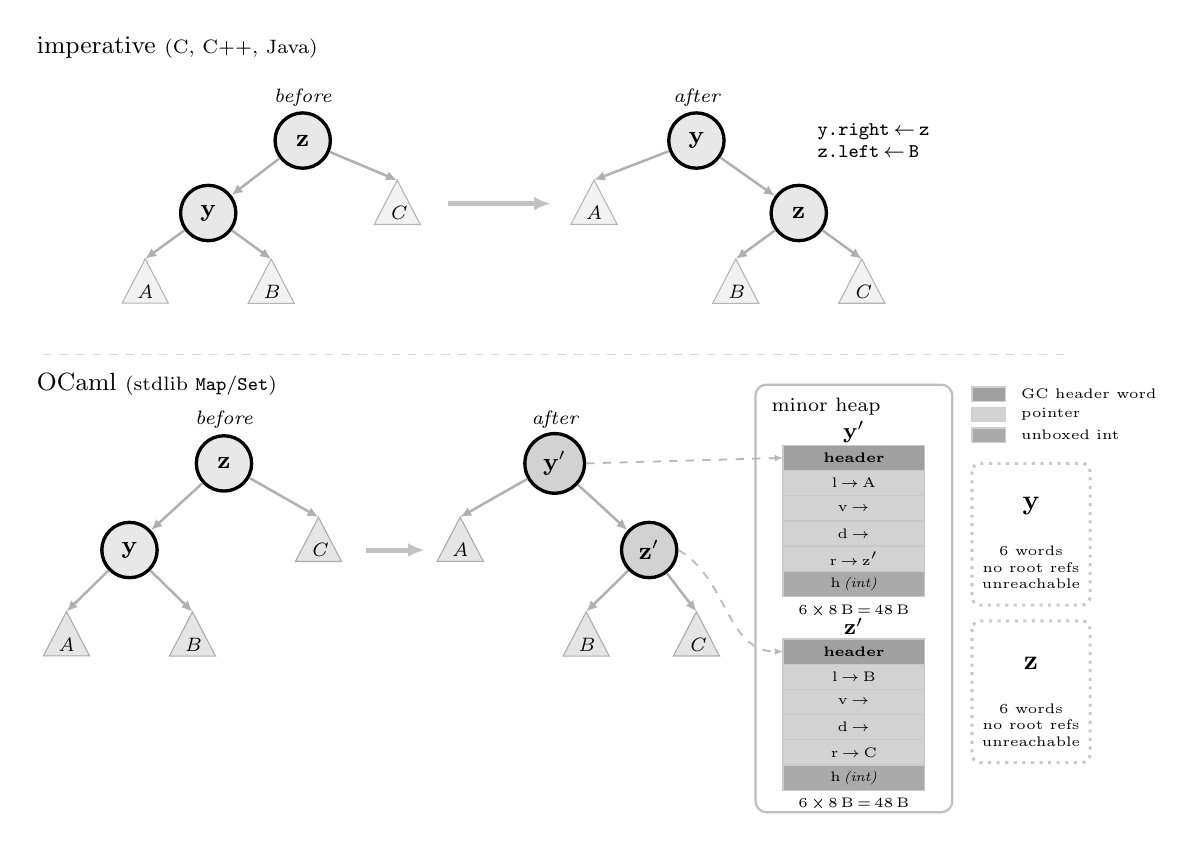
\begin{tikzpicture}

  %%===========================================================================
  %% LAYOUT VARIABLES — adjust these to reposition everything
  %%===========================================================================

  %% ── Heap / legend / old-nodes regions (top-left corner of each) ──────────
  \coordinate (heapbox)  at (9.25,-4);      %% minor heap bounding box
  \coordinate (oldnodes) at (12,-5);      %% old y / z dotted boxes
  \coordinate (legend)   at (12,-4.03);    %% block colour legend

  %% ── Tree root anchors (center of the root node in each tree) ─────────────
  \coordinate (impbefore)  at (3.5,-0.90);   %% imp  before-tree root (z)
  \coordinate (ocalbefore) at (2.5,-5.00);   %% OCaml before-tree root (z)

  %% ── Horizontal gap from before-tree root to after-tree root ──────────────
  \pgfmathsetmacro{\impgap}{5}             %% imperative section gap
  \pgfmathsetmacro{\ocalgap}{4.2}            %% OCaml section gap

  %% After-tree roots are computed from before + gap (same y-level).
  \coordinate (impafter)  at ($(impbefore)+(\impgap, 0)$);
  \coordinate (ocalafter) at ($(ocalbefore)+(\ocalgap,0)$);

  %% ── Section background corners ────────────────────────────────────────────
  %% These derive from tree anchors so backgrounds auto-move with trees.
  %% Tweak the offset constants below if content overflows a background.
  %%
  %%   impbg_TL  = impbefore  + (-4.0, +1.42)   default: (-0.5,  0.52)
  %%   impbg_BR  = impafter   + (+4.8, -2.55)   default: (16.0, -3.45)
  %%   ocalbg_TL = ocalbefore + (-3.0, +1.20)   default: (-0.5, -3.80)
  %%   ocalbg_BR = oldnodes   + (+3.2, -6.45)   default: (16.0,-11.45)
  \coordinate (impbg_TL)  at ($(impbefore)+(-4.0,+1.42)$);
  \coordinate (impbg_BR)  at ($(impafter)+(+4.8,-2.55)$);
  \coordinate (ocalbg_TL) at ($(ocalbefore)+(-3.0,+1.20)$);
  \coordinate (ocalbg_BR) at ($(oldnodes)+(+3.2,-6.45)$);

  %%===========================================================================
  %% SECTION BACKGROUNDS
  %%===========================================================================
  %% backgrounds removed (white on white, were inflating bounding box)

  %% ── Section headers (derived from bg corners) ────────────────────────────
  \node[anchor=west, font=\small, text=black]
  at ($(impbg_TL)+(0.5,-0.24)$)
  {{imperative} \scriptsize (C, C++, Java)%
    % \enspace---\enspace same nodes mutated in place, zero allocation
  };
  \node[anchor=west, font=\small, text=black]
  at ($(ocalbg_TL)+(0.5,-0.20)$)
  {{OCaml} \scriptsize (stdlib \texttt{Map}/\texttt{Set})%
    % \enspace---\enspace immutable; rotation writes two fresh 6-word%
    % records onto the minor heap
  };

  %% ── Dividing line between sections ───────────────────────────────────────
  %% Sits 0.17 below impbg_BR y.  Adjust the -0.17 offset if needed.
  \draw[dashed, gray!30, line width=0.5pt]
  ($(impbg_BR)+(-13.1,-0.17)$) -- ($(impbg_BR)+(-0.1,-0.17)$);

  %%===========================================================================
  %% IMPERATIVE — BEFORE  (right-rotate at z)
  %% All positions are offsets from (impbefore).
  %%===========================================================================
  \node[font=\scriptsize\itshape, black] at
  ($(impbefore)+(0,+0.55)$) {before};

  \node[inode] (zI) at ($(impbefore)+(0,0)$)       {z};
  \node[inode] (yI) at ($(impbefore)+(-1.2,-0.92)$) {y};
  \node[stree] (CI) at ($(impbefore)+(+1.2,-0.92)$) {C};
  \node[stree] (AI) at ($(impbefore)+(-2.0,-1.92)$) {A};
  \node[stree] (BI) at ($(impbefore)+(-0.4,-1.92)$) {B};

  \draw[eptr] (zI) -- (yI);
  \draw[eptr] (zI) -- (CI.apex);
  \draw[eptr] (yI) -- (AI.apex);
  \draw[eptr] (yI) -- (BI.apex);

  \draw[rotarr]
  ($(impbefore)+(1.85,-0.8)$) -- ($(impafter)+(-1.85,-0.8)$);
  % \node[font=\scriptsize, gray!63, align=center]
  % at ($(impbefore)+(3.25,-0.38)$)
  % {right-rotate\\[1pt]{\ttfamily z}};

  %%===========================================================================
  %% IMPERATIVE — AFTER
  %% All positions are offsets from (impafter).
  %%===========================================================================
  \node[font=\scriptsize\itshape, black] at ($(impafter)+(0,+0.55)$) {after};

  \node[inode] (yIA) at ($(impafter)+(0,0)$)       {y};
  \node[stree] (AIA) at ($(impafter)+(-1.3,-0.92)$) {A};
  \node[inode] (zIA) at ($(impafter)+(+1.3,-0.92)$) {z};
  \node[stree] (BIA) at ($(impafter)+(+0.5,-1.92)$) {B};
  \node[stree] (CIA) at ($(impafter)+(+2.1,-1.92)$) {C};

  \draw[eptr] (yIA) -- (AIA.apex);
  \draw[eptr] (yIA) -- (zIA);
  \draw[eptr] (zIA) -- (BIA.apex);
  \draw[eptr] (zIA) -- (CIA.apex);

  \node[font=\scriptsize, black, align=left] at ($(impafter)+(2.25,0)$)
  {
    % same \textbf{y},\,\textbf{z}\enspace---\enspace
    \texttt{y.right}\,$\leftarrow$\,\texttt{z}\\
  \texttt{z.left}\,$\leftarrow$\,\texttt{B}};

  %%===========================================================================
  %% OCAML — BEFORE TREE
  %% All positions are offsets from (ocalbefore).
  %%===========================================================================
  \node[font=\scriptsize\itshape, black] at
  ($(ocalbefore)+(0,+0.55)$) {before};

  \node[inode]  (zO) at ($(ocalbefore)+(0,0)$)       {z};
  \node[inode]  (yO) at ($(ocalbefore)+(-1.2,-1.10)$) {y};
  \node[shtree] (CO) at ($(ocalbefore)+(+1.2,-1.10)$) {C};
  \node[shtree] (AO) at ($(ocalbefore)+(-2.0,-2.30)$) {A};
  \node[shtree] (BO) at ($(ocalbefore)+(-0.4,-2.30)$) {B};

  \draw[eptr] (zO) -- (yO);
  \draw[eptr] (zO) -- (CO.apex);
  \draw[eptr] (yO) -- (AO.apex);
  \draw[eptr] (yO) -- (BO.apex);

  \draw[rotarr]
  ($(ocalbefore)+(1.8,-1.10)$) -- ($(ocalafter)+(-1.65,-1.10)$);
  % \node[font=\scriptsize, gray!63, align=center]
  % at ($(ocalbefore)+(2.75,-0.55)$)
  % {right-rotate\\[1pt]{\ttfamily z}};

  %%===========================================================================
  %% OCAML — AFTER TREE
  %% All positions are offsets from (ocalafter).
  %% y' and z' are new allocations; A, B, C are shared (same heap objects).
  %%===========================================================================
  \node[font=\scriptsize\itshape, black] at ($(ocalafter)+(0,+0.55)$) {after};

  \node[newnode] (yOA) at ($(ocalafter)+(0,0)$)       {y$'$};
  \node[shtree]  (AOA) at ($(ocalafter)+(-1.2,-1.10)$) {A};
  \node[newnode] (zOA) at ($(ocalafter)+(+1.2,-1.10)$) {z$'$};
  \node[shtree]  (BOA) at ($(ocalafter)+(+0.4,-2.30)$) {B};
  \node[shtree]  (COA) at ($(ocalafter)+(+1.8,-2.30)$) {C};

  \draw[nptr] (yOA) -- (AOA.apex);
  \draw[nptr] (yOA) -- (zOA);
  \draw[nptr] (zOA) -- (BOA.apex);
  \draw[nptr] (zOA) -- (COA.apex);

  % \node[font=\tiny, shcol!80, align=center] at ($(ocalbefore)+(2.7,-2.80)$)
  % {A,\,B,\,C shared\enspace---\enspace same heap objects, zero copy};

  %%===========================================================================
  %% MINOR HEAP  (anchored at (heapbox))
  %%
  %% Each Map.Node record has 5 fields + 1 GC header = 6 words × 8 B = 48 B.
  %% Fields: l, v (key), d (val), r  are GC-traced pointers.
  %%         h (height) is an unboxed tagged int — never a GC root.
  %%
  %% Offsets from (heapbox): xl=+0.35  xr=+2.15  xcen=+1.25  block-h=0.32
  %%===========================================================================

  %% ── Minor heap bounding box (stacks are VERTICAL: y' on top, z' below) ──
  \draw[gray!50, line width=0.8pt, rounded corners=4pt]
  ($(heapbox)+(0,0)$) rectangle ($(heapbox)+(2.50,-5.43)$);
  \node[font=\scriptsize, black, anchor=north west]
  at ($(heapbox)+(0.08,-0.04)$) {minor heap};

  %% ── y' stack ────────────────────────────────────────────────────────────
  \node[font=\footnotesize\bfseries, black] at
  ($(heapbox)+(1.25,-0.6)$) {y$'$};

  \filldraw[fill=hdrclr, draw=gray!42, line width=0.45pt]
  ($(heapbox)+(0.35,-0.77)$) rectangle ($(heapbox)+(2.15,-1.09)$);
  \node[font=\tiny\bfseries, black] at ($(heapbox)+(1.25,-0.93)$) {header};

  \filldraw[fill=ptrclr, draw=gray!42, line width=0.45pt]
  ($(heapbox)+(0.35,-1.09)$) rectangle ($(heapbox)+(2.15,-1.41)$);
  \node[font=\tiny, black] at ($(heapbox)+(1.25,-1.25)$) {l\,$\to$\,A};

  \filldraw[fill=ptrclr, draw=gray!42, line width=0.45pt]
  ($(heapbox)+(0.35,-1.41)$) rectangle ($(heapbox)+(2.15,-1.73)$);
  \node[font=\tiny, black] at ($(heapbox)+(1.25,-1.57)$) {v\,$\to$};

  \filldraw[fill=ptrclr, draw=gray!42, line width=0.45pt]
  ($(heapbox)+(0.35,-1.73)$) rectangle ($(heapbox)+(2.15,-2.05)$);
  \node[font=\tiny, black] at ($(heapbox)+(1.25,-1.89)$) {d\,$\to$};

  \filldraw[fill=ptrclr, draw=gray!42, line width=0.45pt]
  ($(heapbox)+(0.35,-2.05)$) rectangle ($(heapbox)+(2.15,-2.37)$);
  \node[font=\tiny, black] at ($(heapbox)+(1.25,-2.21)$) {r\,$\to$\,z$'$};

  \filldraw[fill=intclr, draw=gray!42, line width=0.45pt]
  ($(heapbox)+(0.35,-2.37)$) rectangle ($(heapbox)+(2.15,-2.69)$);
  \node[font=\tiny, black] at ($(heapbox)+(1.25,-2.53)$) {h\,\textit{(int)}};

  \node[font=\tiny, black] at ($(heapbox)+(1.25,-2.87)$)
  {6\,×\,8\,B\,=\,48\,B};

  %% ── z' stack ────────────────────────────────────────────────────────────
  \node[font=\footnotesize\bfseries, black] at
  ($(heapbox)+(1.25,-3.07)$) {z$'$};

  \filldraw[fill=hdrclr, draw=gray!42, line width=0.45pt]
  ($(heapbox)+(0.35,-3.23)$) rectangle ($(heapbox)+(2.15,-3.55)$);
  \node[font=\tiny\bfseries, black] at ($(heapbox)+(1.25,-3.39)$) {header};

  \filldraw[fill=ptrclr, draw=gray!42, line width=0.45pt]
  ($(heapbox)+(0.35,-3.55)$) rectangle ($(heapbox)+(2.15,-3.87)$);
  \node[font=\tiny, black] at ($(heapbox)+(1.25,-3.71)$) {l\,$\to$\,B};

  \filldraw[fill=ptrclr, draw=gray!42, line width=0.45pt]
  ($(heapbox)+(0.35,-3.87)$) rectangle ($(heapbox)+(2.15,-4.19)$);
  \node[font=\tiny, black] at ($(heapbox)+(1.25,-4.03)$) {v\,$\to$};

  \filldraw[fill=ptrclr, draw=gray!42, line width=0.45pt]
  ($(heapbox)+(0.35,-4.19)$) rectangle ($(heapbox)+(2.15,-4.51)$);
  \node[font=\tiny, black] at ($(heapbox)+(1.25,-4.35)$) {d\,$\to$};

  \filldraw[fill=ptrclr, draw=gray!42, line width=0.45pt]
  ($(heapbox)+(0.35,-4.51)$) rectangle ($(heapbox)+(2.15,-4.83)$);
  \node[font=\tiny, black] at ($(heapbox)+(1.25,-4.67)$) {r\,$\to$\,C};

  \filldraw[fill=intclr, draw=gray!42, line width=0.45pt]
  ($(heapbox)+(0.35,-4.83)$) rectangle ($(heapbox)+(2.15,-5.15)$);
  \node[font=\tiny, black] at ($(heapbox)+(1.25,-4.99)$) {h\,\textit{(int)}};

  \node[font=\tiny, black] at ($(heapbox)+(1.25,-5.33)$)
  {6\,×\,8\,B\,=\,48\,B};

  %% ── Arrows: tree nodes → heap stacks ────────────────────────────────────
  \draw[-{Latex[length=3pt,width=2.5pt]}, dashed, line width=0.65pt, gray!55]
  (yOA.east) -- ($(heapbox)+(0.35,-0.93)$);
  \draw[-{Latex[length=3pt,width=2.5pt]}, dashed, line width=0.65pt, gray!55]
  (zOA.east) to[out=-30, in=180] ($(heapbox)+(0.35,-3.39)$);

  %%===========================================================================
  %% UNREACHABLE NODES  (anchored at (oldnodes))
  %% Offsets: center-x=+1.10  right=+2.20
  %%===========================================================================
  % \node[font=\scriptsize, gcred!62, align=center] at
  % ($(oldnodes)+(1.10,0.20)$)
  % {old\enspace\textbf{y},\,\textbf{z}};

  %% old y
  \draw[ogray!50, dotted, line width=1.1pt, rounded corners=3pt]
  ($(oldnodes)+(0,0)$) rectangle ($(oldnodes)+(1.5,-1.8)$);
  \node[font=\normalsize\bfseries, black] at ($(oldnodes)+(0.75,-0.54)$) {y};
  \node[font=\tiny, black, align=center] at ($(oldnodes)+(0.75,-1.32)$)
  {6 words\\no root refs\\unreachable};

  %% old z
  \draw[ogray!50, dotted, line width=1.1pt, rounded corners=3pt]
  ($(oldnodes)+(0,-2)$) rectangle ($(oldnodes)+(1.5,-3.8)$);
  \node[font=\normalsize\bfseries, black] at ($(oldnodes)+(0.75,-2.54)$) {z};
  \node[font=\tiny, black, align=center] at ($(oldnodes)+(0.75,-3.32)$)
  {6 words\\no root refs\\unreachable};

  % \node[font=\scriptsize\bfseries, gcred!70, align=center]
  % at ($(oldnodes)+(1.10,-4.82)$) {$\Rightarrow$ next minor GC};

  %%===========================================================================
  %% BLOCK COLOUR LEGEND  (anchored at (legend))
  %% Offsets: swatch right=+0.42  label x=+0.50  row spacing=0.26
  %%===========================================================================
  \filldraw[fill=hdrclr, draw=gray!38, line width=0.4pt]
  ($(legend)+(0,0)$) rectangle ($(legend)+(0.42,-0.18)$);
  \node[font=\tiny, anchor=west, black] at
  ($(legend)+(0.50,-0.09)$) {GC header word};

  \filldraw[fill=ptrclr, draw=gray!38, line width=0.4pt]
  ($(legend)+(0,-0.26)$) rectangle ($(legend)+(0.42,-0.44)$);
  \node[font=\tiny, anchor=west, black] at ($(legend)+(0.50,-0.35)$) {pointer
  };

  \filldraw[fill=intclr, draw=gray!38, line width=0.4pt]
  ($(legend)+(0,-0.52)$) rectangle ($(legend)+(0.42,-0.70)$);
  \node[font=\tiny, anchor=west, black] at
  ($(legend)+(0.50,-0.61)$) {unboxed int};

\end{tikzpicture}
\end{document}
